%
% 1-definitionen.tex
%
% (c) 2023 Prof Dr Andreas Müller
%
\section{Richtungsableitung und Gradient
\label{buch:fuvar:section:richtungsableitung}}
\kopfrechts{Richtungsableitung und Gradient}
Im Folgenden werden Funktionen betrachtet, die von mehreren unabhängigen
Variablen abhängen.
Solche Funktionen werden $f(x_1,\dots,x_n)$ für die Variablen
$x_1,\dots,x_n$ gesschrieben.
Der Definitionsbereich ist eine Teilmenge $U$ von $\mathbb{R}^n$.
Die reellwertige Funktion
\[
f\colon U\to\mathbb{R} : (x_1,\dots,x_n) \mapsto f(x_1,\dots, x_n)
\]
wird auch abgekürzt $f(x)$ mit $x\in\mathbb{R}^n$ geschrieben.

%
% Partielle Ableitungen
%
\subsection{Partielle Ableitungen}
Die Lösung von Extremalproblemen bei Funktionen einer Variablen
mit Mitteln der Analysis basiert auf der Beobachtung, dass die Ableitung
nach der unabhängigen Variablen verschwinden muss.
Bei einer Funktion mehrere Variablen muss aber erst geklärt werden,
das die Ableitung bei einer Funktion mehrerer Variablen bedeuten soll.

%
% partielle Funktion
%
\subsubsection{Partielle Funktion}
Hält man von einer Funktion $f(x_1,\dots,x_n)$ von den Variablen
$x_1,\dots,x_n$ alle Variablen ausser einer fest, bleibt von $f$ eine
Funktion übrig, die nur noch von dieser einen Variablen abhängt.
Seien also alle Variablen $x_i$ ausser der Variablen $x_k$ fest.
Aus der Funktion $f$ wird damit eine neue Funktion
\[
f_k
\colon
\mathbb{R} \to \mathbb{R}
:
x_k \mapsto f(x_1,\dots,x_k,\dots,x_n).
\]
Die Funktion $f_k$ ist eigentlich eine Funktion, die die festgehaltenen
Variablen als Parameter enthält.
Dies sind die Variablen $x_1,\dots,\widehat{x_k},\dots,x_n$, wobei
wir mit dem Hut anzeigen, dass dieses Element weggelassen werden soll.
Diese Notation wird für alle folgenden Kapitel beibehalten.
Die Funktion $f_k$ wird manchmal auch die {\em partielle Funktion}
\index{partielle Funktion}%
\index{Funktion!partiell}%
genannt.

Unglücklicherweise ist der Begriff der partiellen Funktion auch 
üblich für eine Funktion $A\to B$, die aber nur auf einem Teil
der Menge $A$ definiert ist, deren Definitionsbereich $D(f)$ also
eine echte Teilmenge von $A$ ist.
In diesem Buch ist immer der obengenannte Begriff einer nur von einer
Variablen abhängigen Funktion gemeint.

%
% Ableitungen
%
\subsubsection{Ableitungen}
Da die Funktion $f_k$ nur noch eine Funktion einer einzigen Variablen
ist, ist auch klar, wie sie abgeleitet werden muss.
Die Ableitung von $f_k$ ist
\begin{align*}
\frac{d}{dx_k} f_k(x_k)
&=
\lim_{h\to 0} \frac{f_k(x_k+h)-f_k(x_k)}{h}
\\
&=
\lim_{h\to 0}
\frac{f_k(x_1,\dots,x_k+h,\dots,x_n)-f_k(x_1,\dots,x_k,\dots,x_n)}{h}.
\end{align*}

\begin{definition}
\label{buch:fuvar:richtungsbleitung:def:partielleableitung}
Die {\em partielle Ableitung} einer Funktion $f(x_1,\dots,x_n)$ nach der
\index{partielle Ableitung}%
\index{Ableitung!partiell}%
Variablen $x_k$ ist
\[
\frac{\partial f}{\partial x_k}(x_1,\dots,x_n)
=
\lim_{h\to 0}
\frac{f(x_1,\dots,x_k+h,\dots,x_n)-f(x_1,\dots,x_k,\dots,x_n)}{h}.
\]
Eine Funktion $f(x_1,\dots,x_n)$ heisst {\em stetig differenzierbar}
nach der Variablen $x_k$, wenn die Ableitung der partiellen Funktion 
$f_k$ stetig ist.
\end{definition}

Die partiellen Ableitungen nach einer Variablen entstehen also dadurch,
dass man alle anderen Variablen einer Funktion als konstant betrachtet
und dann die gewöhnliche Ableitung nach der einen verbleibenden Variablen
bildet.

\begin{beispiel}
Die Funktion
\[
f(x,y)
=
\sin(xy)\cos(x+y)
\]
hängt von den Variablen $x$ und $y$ ab.
Die partiellen Funktionen sind
\begin{align*}
x&\mapsto f(x,y)
&&\text{und}&
y&\mapsto f(x,y).
\end{align*}
Zur Berechnung der Ableitungen muss die Produktregel verwendet
werden, sie ergibt die Ableitungen
\begin{align*}
\frac{\partial f}{\partial x}
&=
y\cos(xy)\cos(x+y) -\sin(xy)\sin(x+y)
\\
\frac{\partial f}{\partial x}
&=
x\cos(xy)\cos(x+y) -\sin(xy)\sin(x+y).
\end{align*}
Die beiden Ableitungen unterschieden sich nur in dem Faktor $y$ bzw.~$x$,
der von der inneren Ableitung bei der Ableitung des ersten Faktors
$x\mapsto\sin(xy)$ bzw.~$y\mapsto\sin(xy)$ herrührt.
\end{beispiel}

%
% Partielle Ableitungen als Steigung der Koordinatenlinien
%
\subsubsection{Partielle Ableitungen als Steigungen der Koordinatenlinien}
Der Graph einer Funktion $(x,y)\mapsto f(x,y)$ von zwei Variablen ist 
eine zweidimensionale Fläche über der $x$-$y$-Ebene
(Abbildung~\ref{buch:fuvar:richtungsableitung:fig:partabl}).
%
% partabl.tex -- partielle Ableitungen
%
% (c) 2021 Prof Dr Andreas Müller, OST Ostschweizer Fachhochschule
%
\bgroup
\begin{frame}[t]
\setlength{\abovedisplayskip}{5pt}
\setlength{\belowdisplayskip}{5pt}
\frametitle{Partielle Ableitungen}
\centering
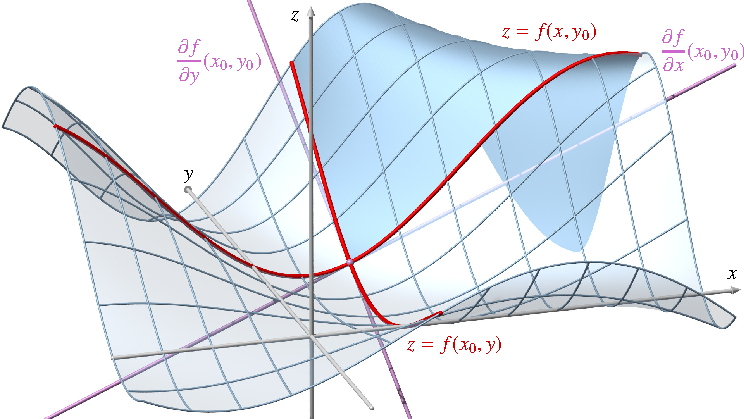
\includegraphics[width=\textwidth]{../slides/1/partabl.pdf}
\end{frame}
\egroup

Die partielle Funktion $x\mapsto f(x,y_0)$ hat als Graph die Schnittkurve
der Fläche mit der vertikalen Ebene $y=y_0$, entsprechend ist der Graph
der partiellen Funktion $y\mapsto f(x_0,y)$ die Schnittkurve der Fläche
mit der vertikalen Ebene $x=x_0$, beide in
Abbildung~\ref{buch:fuvar:richtungsableitung:fig:partabl} blau hervorgehoben.

%
% Notation
%
\subsubsection{Notation}
Die in Definition~\ref{buch:fuvar:richtungsbleitung:def:partielleableitung}
eingeführte Notation ist intuitiv und erinnert an die Notation für den
Differentialquotienten einer Funktion einer Variablen.
Sie hat aber auch einen gravierenden Nachteil, der am Beispiel der
der Funktion $f(x,y)$ illustriert werden soll.
Die partiellen Ableitungen der Funktion $f$ nach $x$ und $y$ sind
\[
\frac{\partial f}{\partial x}
\quad\text{und}\qquad
\frac{\partial f}{\partial y}.
\]
Setzt man die Argumentwerte $x^2+y^2$ und $x^2-y^2$ in die Funktion
$f$ ein, entsteht dann die Funktion
\begin{equation}
(x,y) \mapsto f(x^2+y^2,x^2-y^2).
\label{buch:fuvar:richtungsableitung:eqn:feingesetzt}
\end{equation}
Wie soll man die Ableitung dieser Funktion nach $x$ schreiben?
Und was soll die Notation
\[
\frac{\partial f}{\partial x}(x^2+y^2,x^2-y^2)
\]
bedeuten?
Ist dies die partielle Ableitung nach dem ersten Argument von $f$
oder ist es die Ableitung der zusammengesetzten Funktion nach $x$?

Offenbar wurden hier die Symbole $x$ und $y$ auf zwei verschiedene
Arten verwendet.
In der Schreibweise $f(x,y)$ ist das $x$ ein Platzhalter für die
erste Variable, das $y$ ist Platzhalter für die zweite Variable.
Die Symbole haben also vor allem syntaktische Eigenschaften.
Die Aussage, dass $f$ eine Funktion $\mathbb{R}^2\to\mathbb{R}$
ist, sagt genauso viel.
Die Variablen $x$ und $y$ werden nur gebraucht, wenn man zum
Beispiel mit einer Formel wie $f(x,y)=\sin x\cdot\cos y$ 
anzeigen will, wie ein Funktionswert berechnet werden soll.

In der Form~\eqref{buch:fuvar:richtungsableitung:eqn:feingesetzt} ist
stehen aber $x$ und $y$ für beliebige reelle Zahlen.
Daraus müssen erst die Werte $x^2+y^2$ und $x^2-y^2$ berechnet werden,
die dann als erstes bzw.~zweites Argument der Funktion eingesetzt
werden müssen.
Die Notation~\eqref{buch:fuvar:richtungsableitung:eqn:feingesetzt} ist also
eigentlich eine abgekürzte Schreibweise für eine zusammengesetzte
Funktion, die sich aus
\[
g
\colon
\mathbb{R}^2 \to \mathbb{R}^2
:
(x,y) \mapsto (x^2+y^2,x^2-y^2)
\]
und der Funktion $f$ zusammensetzt.

\begin{beispiel}
\label{buch:fuvar:richtungsableitung:bsp:L}
In Abschnitt~\ref{buch:variation:section:eulerlagrange} werden wir
Extremalprobleme für Funktionen konstruieren, die als Integrale
einer Funktion $L$ von drei Variablen entstehen.
Zu jeder Funktion $y\colon \mathbb{R}\to\mathbb{R}:x\mapsto y(x)$
wird das Integral
\begin{equation*}
I
=
\int_a^b L(x,y(x),y'(x))\,dx
\end{equation*}
berechnet.
Die Funktion $L$ wird dabei meistens als $L(x,y,y')$ geschrieben.
Es wird dann die  Euler-Lagrange-Differentialgleichung abgeleitet,
in der die Ausdrücke
\begin{equation}
\frac{\partial L}{\partial y}
\qquad\text{und}\qquad
\frac{\partial L}{\partial y'}
\label{buch:fuvar:richtungsableitungen:eqn:Lderiv}
\end{equation}
auftreten.
Obwohl $y$ und $y'$ Funktionen von $x$ sind, sind mit den 
partiellen Ableitungen~\eqref{buch:fuvar:richtungsableitungen:eqn:Lderiv}
die Ableitungen nach der zweiten und dritten unabhängigen Variable
von $L$ gemeint.
\end{beispiel}

\begin{definition}
\label{buch:fuvar:richtungsableitung:def:D}
Sei $f\colon \mathbb{R}^n \to V$ eine Funktion von $n$ Variablen
mit Werten in einem endlichdimensionalen Vektorraum.
Die partielle Ableitung nach der $k$-ten Variable wird auch als
\[
D_kf(x_1,\dots,x_n)
=
\lim_{h\to 0}
\frac{f(x_1,\dots,x_k+h,\dots,x_n)-f(x_1,\dots,x_k,\dots,x_n)}{h}
\]
bezeichnet.
\end{definition}

\begin{beispiel}
Mit der Notation von Definition~\ref{buch:fuvar:richtungsableitung:def:D}
werden die partiellen Ableitungen der Funktion $L(x,y,y')$ von
Beispiel~\ref{buch:fuvar:richtungsableitung:bsp:L} zu
\begin{align*}
\frac{\partial L}{\partial x}(x,y,y')
&=
D_1L(x,y,y'),
\\
\frac{\partial L}{\partial y}(x,y,y')
&=
D_2L(x,y,y')
\intertext{und}
\frac{\partial L}{\partial y'}(x,y,y')
&=
D_3L(x,y,y').
\end{align*}
Die neue Notation eliminiert die Zweideutigkeit.
$D_3L(x,y(x),y'(x))$ bedeutet, dass die Funktion $L$ zuerst partiell
nach der dritten Variable abgeleitet werden soll, dann sollen die
Werte $x$, $y(x)$ und $y'(x)$ als Argumente eingesetzt werden.
\end{beispiel}

%
% Lineare Ersatzfunktion
%
\subsubsection{Lineare Ersatzfunktion}
%
% tangentialebene.tex
%
% (c) 2024 Prof Dr Andreas Müller
%
\begin{figure}
\centering
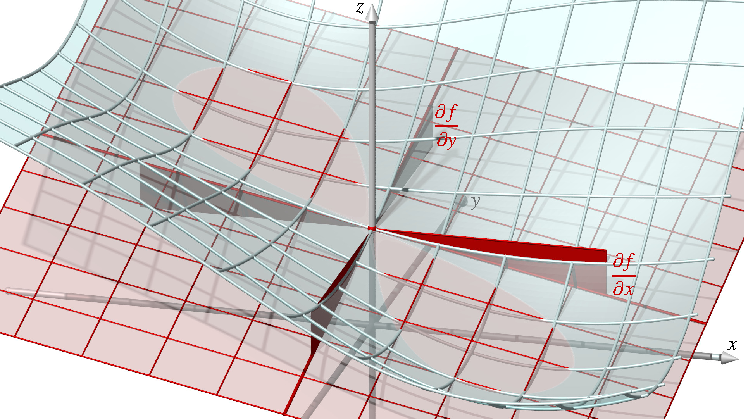
\includegraphics{chapters/010-fuvar/images/tangential.pdf}
%\includegraphics{chapters/010-fuvar/images/tangentialebene.pdf}
\caption{Mit den partiellen Ableitungen $\frac{\partial f}{\partial x}$
und $\frac{\partial f}{\partial y}$ einer Funktion lässt sich die rote
Tangentialebene in einem Punkt als lineare Ersatzfunktion konstruieren.
\label{buch:fuvar:richtungsableitung:fig:tangentialebene}}
\end{figure}

Die Ableitung einer Funktion wird manchmal auch als eine lineare
Ersatzfunktion definiert.

\begin{definition}
Eine Funktion $f\colon\mathbb{R}^n\to\mathbb{R}^m$ heisst differenzierbar
im Punkt $x_0\in\mathbb{R}^n$, wenn es eine lineare Funktion
$l\colon \mathbb{R}^n\to\mathbb{R}^m$ gibt mit der Eigenschaft, dass
\[
|f(x_0+x) - f(x_0) - l(x)| = o(x)h
\]
ist.
Diese Notation bedeutet, dass
\[
\lim_{x\to 0}
\frac{|f(x_0+x)-f(x_0)-l(x)|}{|x|}
=
0.
\]
Man sagt auch, eine $o(x)$-Funktion geht schneller gegen $0$ als $x$.
\end{definition}

%
% Kettenregel
%
\subsubsection{Kettenregel}
Die Kettenregel ermöglich, die Ableitungen zusammengestzter Funktionen
zu berechnen.
Im vorliegenden Kontext der Funktionen mehrerer Variablen suchen
wir nach einer Regel, die Ableitungen einer zusammengesetzten Funktion
$f\circ g$ berechnet für zwei Funktionen
\[
g\colon \mathbb{R}^r\to\mathbb{R}^n
\qquad\text{und}\qquad
f\colon \mathbb{R}^n\to\mathbb{R}^m.
\]
Die lineare Ersatzfunktion der Funktion $g$ ist jetzt eine Matrix.

\begin{definition}
\label{buch:fuvar:richtungsableitung:def:ableitungsmatrix}
Die partiellen Ableitungen einer Funktion
$g\colon\mathbb{R}^n\to\mathbb{R}^m$
kann als $m\times n$-Matrix
\[
Dg
=
\begin{pmatrix}
D_1g_1 & D_2g_1 & \dots  & D_ng_1 \\
D_1g_2 & D_2g_2 & \dots  & D_ng_2 \\
\vdots & \vdots & \ddots & \vdots \\
D_1g_m & D_2g_m & \dots  & D_ng_m
\end{pmatrix}
=
J_g
=
{\renewcommand{\arraystretch}{1.3}
\begin{pmatrix}
\frac{\partial g_1}{\partial x_1}
	& \frac{\partial g_1}{\partial x_2}
		&\dots
			&\frac{\partial g_1}{\partial x_n}
\\
\frac{\partial g_2}{\partial x_1}
	& \frac{\partial g_2}{\partial x_2}
		&\dots
			&\frac{\partial g_2}{\partial x_n}
\\
\vdots	&\vdots	&\ddots	&\vdots \\
\frac{\partial g_m}{\partial x_1}
	& \frac{\partial g_m}{\partial x_2}
		&\dots
			&\frac{\partial g_m}{\partial x_n}
\end{pmatrix}}
\]
gesschrieben werden.
Sie heisst auch die {\em Jacobi-Matrix}.
\index{Jacobi-Matrix}%
\end{definition}

Die Ableitung einer zusammengesetzten Funktion $f(g(x))$ einer 
Variable ist durch die Kettenregel
\[
(f\circ g)'(x)
=
f'(g(x)) g'(x)
\]
gegeben.
Für Funktionen mehrerer Variablen wird die Formel etwas komplizierter.

\begin{satz}
Seien $f\colon \mathbb{R}^m\to\mathbb{R}^n$ und
$g\colon\mathbb{R}^r\to\mathbb{R}^m$ Funktionen und sei zudem
$g$ im Punkt $x_0$ differenzierbar und $f$ im Punkt $g(x_0)$.
Dann ist die Zusammensetzung $f\circ g$ differenzierbar im Punkt $x_0$
und die Ableitungsmatrix ist
\[
D(f\circ g) = Df(g(x_0)) Dg(x_0).
\]
\end{satz}

Schreibt man $g(x)=y\in\mathbb{R}^m$ und ist $f(y)$ eine reellwertige Funktion
mit den partiellen Ableitungen
\[
D_k(f\circ g)(x)
=
D_kf(g(x_0)) Dg(x_0)
=
\sum_{l=1}^n
\frac{\partial f}{\partial y_l}(g(x_0))
\frac{\partial y_l}{\partial x_k}(x_0).
\]

%
% Höhere Ableitungen
%
\subsubsection{Höhere Ableitungen}
Ist $f\colon U\to\mathbb{R}$ eine differenzierbare Funktion, dann ist
die Ableitung
\[
\partial_if\colon x\mapsto \frac{\partial f}{\partial x_i}(x)
\]
wieder eine stetige Funktion auf $U$, und man kann erneut die Frage
stellen, ob sie differenzierbar ist.
Die folgende rekursive Definition schafft einen handlichen Begriff
dafür.

\begin{definition}[Höhere partielle Ableitungen]
Eine Funktion $f\colon U\to\mathbb{R}$ mit $U\subset\mathbb{R}^n$ heisst
{\em $n$ mal differenzierbar}, wenn die partiellen Ableitungen
\[
\partial_i f
\colon
U\to\mathbb{R}
:
x\mapsto
\frac{\partial f}{\partial x_i}(x)
\]
für alle $i=1,\dots,n$ $n-1$-mal differenzierbar sind.
Sie heisst {\em $n$-mal stetig} differenzierbar, wenn alle partiellen
ersten Ableitungen $n-1$-mal stetig differenzierbar sind.
\end{definition}

Wenn eine Funktion zweimal differenzierbar ist, existieren alle
partiellen Ableitungen
\[
\frac{\partial^2 f}{\partial x_i\,\partial x_k},
\quad
i,k=1,\dots,n,
\]
es ist aber a priori alles andere als klar, ob die Reihenfolge der
Ableitungen eine Rolle spielt.
Der folgende Satz von Schwarz klärt diese Frage.

\begin{satz}[Schwarz]
Ist $f\colon U\to\mathbb{R}$ für eine offene Umgebung $U\subset\mathbb{R}^n$
eine zweimal stetig differenzierbare Funktion, dann kommt es bei
gemischten Ableitungen nicht auf die Reihenfolge an, es ist
\[
\frac{\partial^2 f}{\partial x_i\,\partial x_k}(x)
=
\frac{\partial^2 f}{\partial x_k\,\partial x_i}(x)
\]
für alle $x\in U$.
\end{satz}

Man beachte, dass der Satz nicht gilt, wenn die Ableitungen nur
existieren, aber nicht notwendigerweise stetig sind.
In diesem Fall lassen sich Gegenbeispiele konstruieren, wie
das folgende Beispiel von Schwarz zeigt.

\begin{beispiel}
\label{buch:fuvar:richtungsableitung:beispiel:schwarz}
%
% schwarz.tex -- Gegenbeispiel zum Satz von Schwarz
%
% (c) 2024 Prof Dr Andreas Müller
%
\begin{figure}
\centering
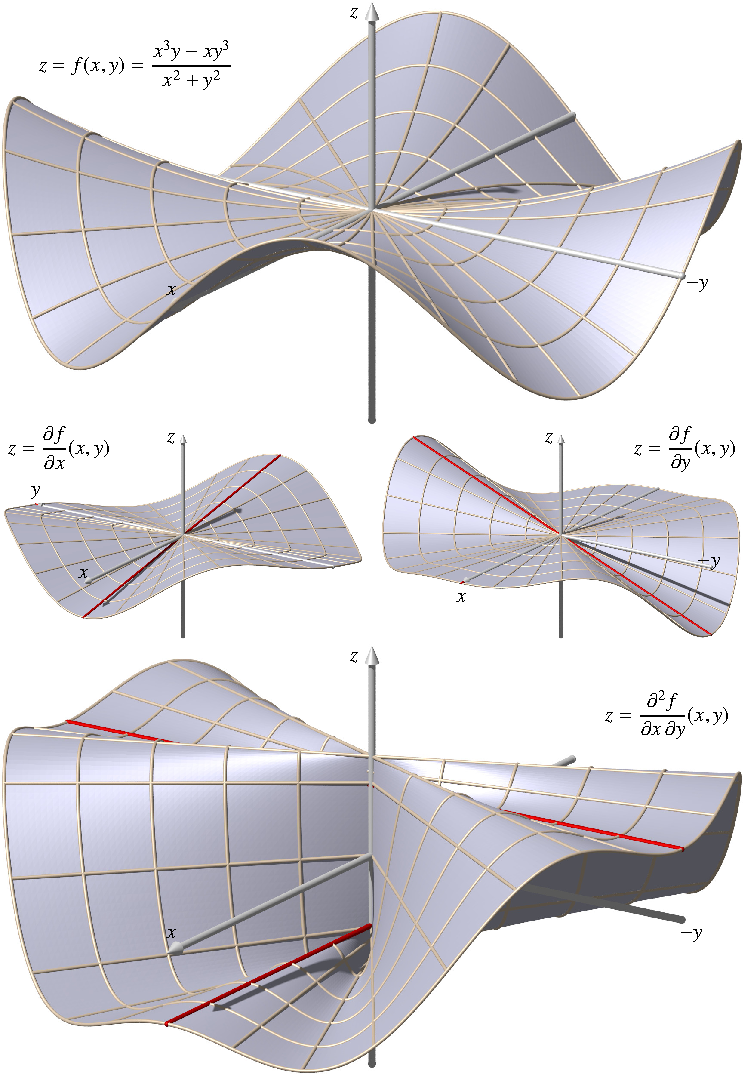
\includegraphics{chapters/010-fuvar/images/schwarz.pdf}
\caption{Gegenbeispiel~\ref{buch:fuvar:richtungsableitung:beispiel:schwarz}
zum Satz von Schwarz.
Oben der Graph der Funktion $f(x,y)$, in der Mitte die beiden 
ersten partiellen Ableitungen.
Die gemischten Ableitungen in der untersten Abbildung ist an der
Stelle $(x,y)=(0,0)$ nicht mehr stetig.
\label{buch:fuvar:richtungsableitung:fig:schwarz}}
\end{figure}

Wir betrachten die Funktion
\[
f
\colon
\mathbb{R}^2\to\mathbb{R}
:
(x,y)
\mapsto
f(x,y)
=
\begin{cases}
\displaystyle \frac{x^3y-xy^3}{x^2+y^2}&\qquad (x,y)\ne (0,0)\\
(0,0)&\qquad\text{sonst},
\end{cases}
\]
die auch in Abbildung~\ref{buch:fuvar:richtungsableitung:fig:schwarz}
zusammen mit den partiellen ersten Ableitungen und den gemischten
zweiten Ableitungen dargestellt ist.
Die Ableitungen im Nullpunkt sind
\begin{align*}
\frac{\partial f}{\partial x}(x,y)
&=
\frac{x^4y+4x^2y^3-y^5}{(x^2+y^2)^2}
&&\Rightarrow&
\frac{\partial f}{\partial x}(0,y)
&=
\frac{-y^5}{y^4} = -y
\\
\frac{\partial f}{\partial y}(x,y)
&=
\frac{x^5-4x^3y^2-xy^4}{(x^2+y^2)^2}
&&\Rightarrow&
\frac{\partial f}{\partial y}(x,0)
&=
\frac{x^5}{x^4}
=
x.
\intertext{Sie sind in Abbildung~\ref{buch:fuvar:richtungsableitung:fig:schwarz}
in der Mitte rot hervorgehoben.
Daraus ergeben sich die zweiten Ableitungen}
\frac{\partial^2 f}{\partial y\,\partial x}(0,y)
&=
\frac{\partial}{\partial y}(-y)
=
-1
&&\Rightarrow&
\frac{\partial^2 f}{\partial y\,\partial x}(0,0)
&=
-1
\\
\frac{\partial^2 f}{\partial x\,\partial y}(x,0)
&=
\frac{\partial}{\partial x}(x)
=
1
&&\Rightarrow&
\frac{\partial^2 f}{\partial x\,\partial y}(0,0)
&=
1.
\end{align*}
Die erste Gleichung entspricht den roten Geraden über der $y$-Achse
in Abbildung~\ref{buch:fuvar:richtungsableitung:fig:schwarz},
die zweite entspricht den roten Geraden über der $x$-Achse.
Die roten Geraden zeigen daher gemischte zweite Ableitungen in
verschiedenen Differentiationsreihenfolgen mit verschiedenen
Werten.
Somit sind die Grenzwerte an der Stelle $(0,0)$ verschieden und
die Funktion der gemischten Ableitungen ist nicht stetig an der Stelle
$(0,0)$.

Die Abbildung~\ref{buch:fuvar:richtungsableitung:fig:schwarz}
zeigt auch, dass der Funktionsgraph sowohl von $\frac{\partial f}{\partial x}$
und $\frac{\partial f}{\partial y}$ im Nullpunkt keine lineare
Ersatzfunktion hat.
\end{beispiel}

%
% Richtungsableitung
%
\subsection{Richtungsableitung}
Die partiellen Ableitungen einer Funktion $f(x_1,\dots,x_n)$
nach der Variablen $x_k$ entstehen dadurch, dass alle Variablen
ausser $x_k$ konstant gehalten werden und die so entstehende
Funktion der einzigen Variablen $x_k$ abgeleitet wird.
%
% richtungsableitung.tex -- Richtungsableitung einer Funktion f(x,y)
%
% (c) 2024 Prof Dr Andreas Müller
%
\begin{figure}
\centering
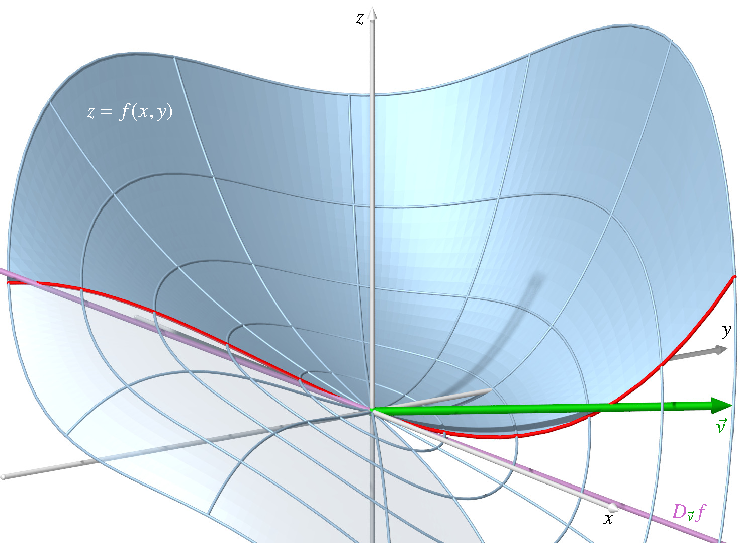
\includegraphics{chapters/010-fuvar/images/richtungsabl.pdf}
\caption{Definition der Richtungsableitung einer Funktion $f(x,y)$
zweier Variablen in Richtung des {\color{darkgreen}grünen}
Vektors ${\color{darkgreen}\vec{v}}$.
Die Richtungsableitung ist die Steigung der {\color{darkred}roten}
Schnittkurve der vertikalen Ebene mit Richtung ${\color{darkgreen}\vec{v}}$ 
und der Fläche des Graphen $z=f(x,y)$.
\label{buch:fuvar:richtungsableitung:fig:richtungsableitung}}
\end{figure}

%
% partrichtung.tex
%
% (c) 2024 Prof Dr Andreas Müller
%
\begin{figure}
\centering
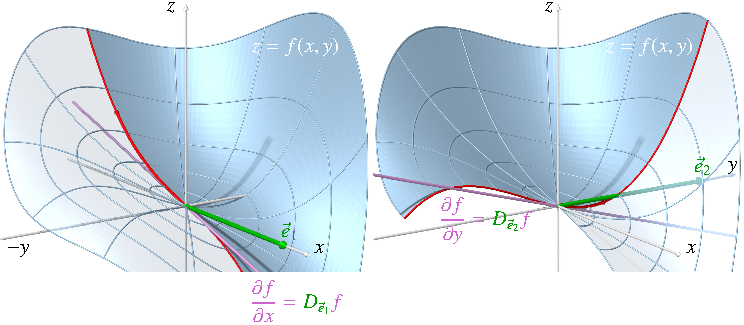
\includegraphics{chapters/010-fuvar/images/fxy.pdf}
\caption{Die partiellen Ableitungen sind Richtungsableitungen der
Funktion in Richtung der Koordinatenachsen.
\label{buch:fuvar:richtungsableitung:fig:partrichtung}}
\end{figure}

Die Funktion $f$ kann aber noch auf eine andere Art zu einer
Funktion nur einer Variablen gemacht werden.
Dazu verwendet man die Parameterdarstellung $x(t) = x + vt$ einer
Geraden durch den Punkt $x$ mit Richtungsvektor $v$
(Abbildung~\ref{buch:fuvar:richtungsableitung:fig:richtungsableitung}).
Die Funktion $f(x+vt)$ hängt nur noch von der Variablen $t$ ab
und kann wie gewohnt nach $t$ abgeleitet.

\begin{definition}
\label{buch:fuvar:richtungsableitung:def:richtungsableitung}
Die {\em Richtungsableitung} der Funktion $f\colon\mathbb{R}^n\to\mathbb{R}^m$
\index{Richtungsableitung}%
im Punkt $x\in\mathbb{R}^n$ in Richtung $v\in\mathbb{R}^n$ ist 
\[
D_vf(x)
=
\frac{d}{dt}f(x+tv)\bigg|_{t=0}.
\]
\end{definition}

Die Notation für die Richtungsableitung von
Definition~\ref{buch:fuvar:richtungsableitung:def:richtungsableitung}
konkurriert mit der Notation für die partiellen Ableitungen von
Definition~\ref{buch:fuvar:richtungsableitung:def:D}.
Tatsächlich entsteht aber kein Widerspruch, denn die 
Richtungsableitung in Richtung des Standardbasisvektors $e_k$ ist
\begin{align*}
D_{e_k}f(x)
&=
\frac{d}{dt} f(x+te_k)\bigg|_{t=0}
\\
&=
\lim_{h\to 0}
\frac{f(x_1,\dots,x_k+t,\dots,x_n)-f(x_1,\dots,x_k,\dots,x_n)}{h}
\\
&=
D_kf(x)
\end{align*}
oder kurz $D_{e_k}=D_k$
(siehe auch Abbildung~\ref{buch:fuvar:richtungsableitung:fig:partrichtung}).

Die Ableitung der Funktion $t\mapsto x+vt$ für $x\in\mathbb{R}^n$
und $v\in\mathbb{R}^n$ nach der einen Variablen $t$ ist
\[
\frac{d}{dt}
\begin{pmatrix}
x_1+v_1t\\
x_2+v_2t\\
\vdots  \\
x_n+v_nt
\end{pmatrix}
=
\begin{pmatrix}
v_1\\
v_2\\
\vdots\\
v_n
\end{pmatrix}.
\]
Damit kann die Richtungsableitung einer Funktion
$f\colon\mathbb{R}^n\to\mathbb{R}$
im Punkt $x\in\mathbb{R}^n$ kann mit der Kettenregel als
\begin{equation}
D_vf(x)
=
\frac{\partial f}{\partial x_1}(x) v_1
+
\dots
+
\frac{\partial f}{\partial x_n}(x) v_n
=
\sum_{k=1}^n \frac{\partial f}{\partial x_k} v_k
\label{buch:fuvar:richtungsableitung:eqn:richtungsableitungkette}
\end{equation}
berechnet werden.

%
% Gradient
%
\subsection{Gradient}
Die Schreibweise
\eqref{buch:fuvar:richtungsableitung:eqn:richtungsableitungkette}
für die Richtungsableitung der Funktion $f\colon\mathbb{R}^n\to\mathbb{R}$
lässt sich auch als Skalarprodukt des Vektors $v$ mit einem Vektor
bestehend aus den partiellen Ableitungen schreiben.

\begin{definition}
\label{buch:fuvar:richtungsableitung:def:gradient}
Der {\em Gradient} der Funktion $f\colon\mathbb{R}^n\to\mathbb{R}$ ist der
Vektor
\[
\operatorname{grad}f(x)
=
{
\renewcommand{\arraystretch}{1.9}
\begin{pmatrix}
\displaystyle
\frac{\partial f}{\partial x_1}(x)\\
\displaystyle
\frac{\partial f}{\partial x_2}(x)\\
\vdots \\
\displaystyle
\frac{\partial f}{\partial x_n}(x)
\end{pmatrix}
}
\]
\index{Gradient}
\end{definition}

Der Gradient ist auch die transponierte Matrix der Jacobi-Matrix:
$\operatorname{grad}f(x) = \transpose{Df(x)} = \transpose{J_f(x)}$.
Als weitere Notation ist ausserdem der Nabla-Operator gemäss der folgenden
Definition verbreitet.

\begin{definition}[Nabla-Operator]
\label{buch:fuvar:richtungsableitung:def:nabla}
Der {\em Nabla-Operator} ist der Differentialoperator
\index{Nabla-Operator}%
\index{Operator!Nabla-}%
\[
\nabla 
=
{
\renewcommand{\arraystretch}{1.8}
\begin{pmatrix}
\displaystyle
\frac{\partial}{\partial x_1}\\
\displaystyle
\frac{\partial}{\partial x_2}\\
\vdots\\
\displaystyle
\frac{\partial}{\partial x_n}
\end{pmatrix}
}
\]
auf Funktionen
$\mathbb{R}^n\to\mathbb{R}$, der durch
\[
\nabla f
=
{
\renewcommand{\arraystretch}{1.9}
\begin{pmatrix}
\displaystyle
\frac{\partial f}{\partial x_1}(x)\\
\displaystyle
\frac{\partial f}{\partial x_2}(x)\\
\vdots\\
\displaystyle
\frac{\partial f}{\partial x_n}(x)
\end{pmatrix}
}
=
\operatorname{grad}f(x)
\]
definiert ist.
\end{definition}



